\documentclass[tikz]{standalone}
\usepackage{tikz}
\usetikzlibrary{calc,positioning, shapes, petri, automata}
\tikzset{
    transV/.style={transition, fill=black, minimum height = 12mm, minimum width = 1.5mm,inner sep = 0mm},
    transH/.style={transition, fill=black, minimum width = 12mm, minimum height = 1.5mm,inner sep = 0mm},
    node distance=1.5
}
\usepackage{amsmath,amssymb,amsthm,mathrsfs,amsfonts}

\usepackage{csquotes}
\usepackage{booktabs}

\usepackage{graphicx}
\graphicspath{ {../img/} }

\newcommand{\LSset}[2]{\scriptsize $\begin{aligned}&\{#1\}_L\\&\{#2\}_S\end{aligned}$}


\begin{document}    
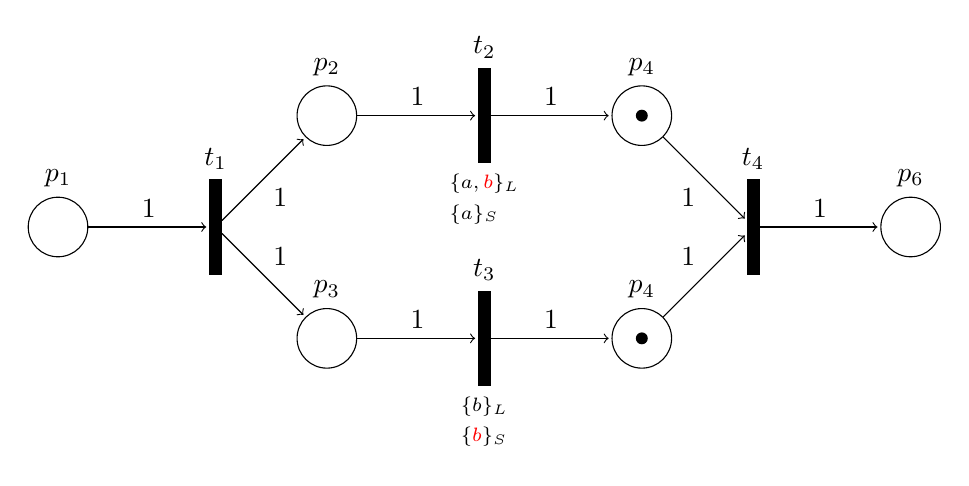
\begin{tikzpicture}[node distance=2cm,on grid, auto]
  \node[place, label=$p_1$] (p1) {};
  \node[transV, label=$t_1$, right = of p1] (t1) {};
  \node[place, label=$p_2$, above right = of t1] (p2) {};
  \node[place, label=$p_3$, below right = of t1] (p3) {};
  \node[transV,label=$t_2$, right = of p2,label=below:{\LSset{a,{\color{red}b}}{a}} ] (t2){};
  \node[transV,label=$t_3$, right = of p3,label=below:{\LSset{b}{{\color{red}b}}}] (t3){};
  \node[place, label=$p_4$, tokens=1, right = of t2] (p4) {};
  \node[place, label=$p_4$, tokens=1, right = of t3] (p5) {};
  \node[transV, label=$t_4$, below right = of p4] (t4) {};
  \node[place, label=$p_6$, right = of t4] (p6) {};



  \draw 
  (p1) edge[post] node {1} (t1)
  (t1) edge[post] node [swap] {1} (p2)
  (t1) edge[post] node {1} (p3)
  (p2) edge[post] node {1} (t2)
  (p3) edge[post] node {1} (t3)
  (t2) edge[post] node {1} (p4)
  (t3) edge[post] node {1} (p5)
  (p4) edge[post] node [swap] {1} (t4)
  (p5) edge[post] node {1} (t4)
  (t4) edge[post] node {1} (p6)
  ;
\end{tikzpicture}
\end{document}